%------------------------------------------------
%	PACKAGES AND DOCUMENT CONFIGURATIONS
%------------------------------------------------
\documentclass[11pt]{article}
\usepackage{amsmath} % Required for some math elements
\usepackage{hyperref} 
\usepackage{xcolor}
\usepackage{lipsum} 
\usepackage{cite}
\usepackage{graphicx} % Required for the inclusion of images
\usepackage{algorithmic}
\usepackage{array}
\usepackage{bookmark}
\usepackage{listings}
\usepackage{amssymb}
\usepackage{enumitem}
\usepackage{pythonhighlight}
\usepackage[T1]{fontenc}
\usepackage{inconsolata}
\usepackage[margin=16mm]{geometry}
\usepackage[caption=false, font=footnotesize]{subfig}
\usepackage[active,tightpage]{preview}

\renewcommand{\PreviewBorder}{1in}
\newcommand{\Newpage}{\end{preview}\begin{preview}}

\newlist{steps}{enumerate}{1}
\setlist[steps, 1]{label = Step \arabic*:}

\hypersetup{ %color attributes of citation, link, etc.
    colorlinks=true,
    linkcolor=blue,
    filecolor=gray,      
    urlcolor=blue,
    citecolor=blue,
}

\newcommand{\matlab}{\textsc{Matlab }} %very important and totally necessary addition

\newcommand\Item[1][]{%
  \ifx\relax#1\relax  \item \else \item[#1] \fi
  \abovedisplayskip=0pt\abovedisplayshortskip=0pt~\vspace*{-\baselineskip}}

%----------------------------------
%	DOCUMENT INFORMATION
%----------------------------------
 
\title{ECEN321 : Estimation \\ Lab 3 Submission}
\author{Daniel Eisen : 300447549}
\date{\today}

\begin{document}
\begin{preview}
\maketitle
%-----------------------------
%	DOCUMENT CONTENT
%-----------------------------
\section{Introduction}
This lab is covers methods of fitting real world dataset to theoretical distributions. This necessitates analysing the dataset and estimating the parameters of the distribution that represents the signal. This lab specifically covers the effect of the number of realisations on the precision and accuracy of the parameter estimation; and a numerical parameter estimation of a real world signals.
\section{Theory}
\subsubsection*{Part 1}
Estimation base on N realisations:\\

The estimator $\bar{X}$ of the population mean $\mu$ is unbiased and its variance is equal to $\frac{\sigma^2}{N}$. So as we sample from a greater N of realisations the variance in the estimated mean will decrease, but even for low N the distribution in these estimations will still be centred on the true mean.\\

The estimator of the population $sigma^2$ is $s^2$.
Due to these samples being taken from a normal distribution we can say that $\frac{N-1}{\sigma^2}S^2$ is equal to the Chi-squared distribution with $n-1$ degrees of freedom. So as more realisations are taken, N increases, the distribution in of the estimated variance becomes more normally distributed; just as the Chi-squared with increasing degrees of freedom.


\subsubsection*{Part 2}
The samples in the signal are in reality not independent, but they are more dependant the closer they are. So for a signal of larger length such as this we can treat all samples are independent without such a great impact on the analysis, and in parameter estimation. \\

For the estimation we take the Likelihood function of the Generalised Normal Distribution, which we use the log of due to break down in computer precision and maximise its output for a range of alpha and beta values, repeating this until convergence.
\begin{align*}
        \mathrm{Generalised\;Normal\;Distribution} \\
        f(x;\alpha,\beta,\mu) &= \frac{\beta}{2\alpha\Gamma(1/\beta)}e^{-(|x-\mu|\alpha)^\beta}\\ \\
        \mathrm{Likelihood\;Equation}\\ 
        L(\alpha, \beta ; x) &= \prod^N_{i=1} \frac{\beta}{2\alpha\Gamma(\frac{1}{\beta})} e^{-(\frac{|x-\mu|}{\alpha})^\beta}\\
        -ln (L(\alpha, \beta ; x)) &= \sum^N_{i=1} -ln\left(\frac{\beta}{2\alpha\Gamma(\frac{1}{\beta})}\right) + \sum^N_{i=1} -ln(e^{-(\frac{|x-\mu|}{\alpha})^\beta})\\\\
         &= N\left(ln\left(\frac{\beta}{2\alpha\Gamma(\frac{1}{\beta})}\right)\right) - \sum^N_{i=1} \left( \frac{|x-\mu|}{\alpha}\right)^\beta \\
         &= N(ln(\beta)) - ln(2\alpha) - ln(\Gamma(\frac{1}{\beta})) - \sum^N_{i=1} \left( \frac{|x-\mu|}{\alpha}\right)^\beta\\
\end{align*} 

\section{Results}
\subsubsection*{Part 1}
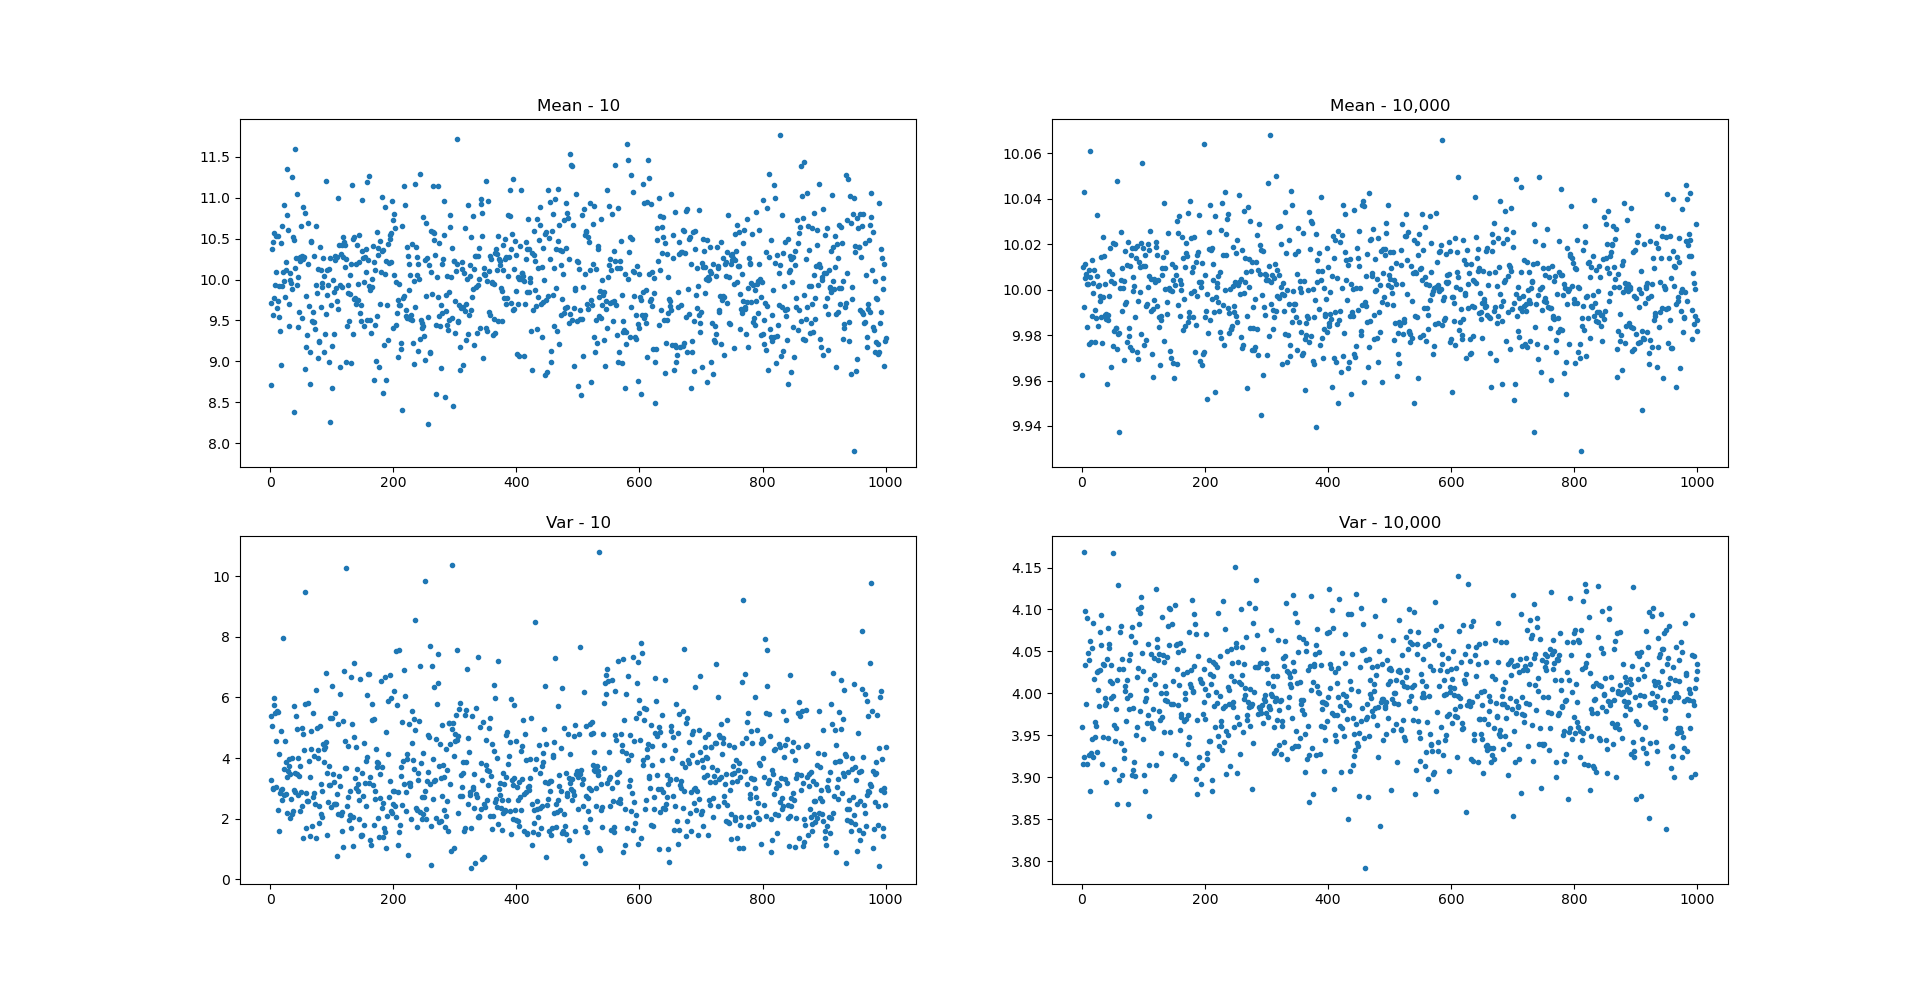
\includegraphics[width = 0.5\textwidth]{inc/p1_scatter.png}
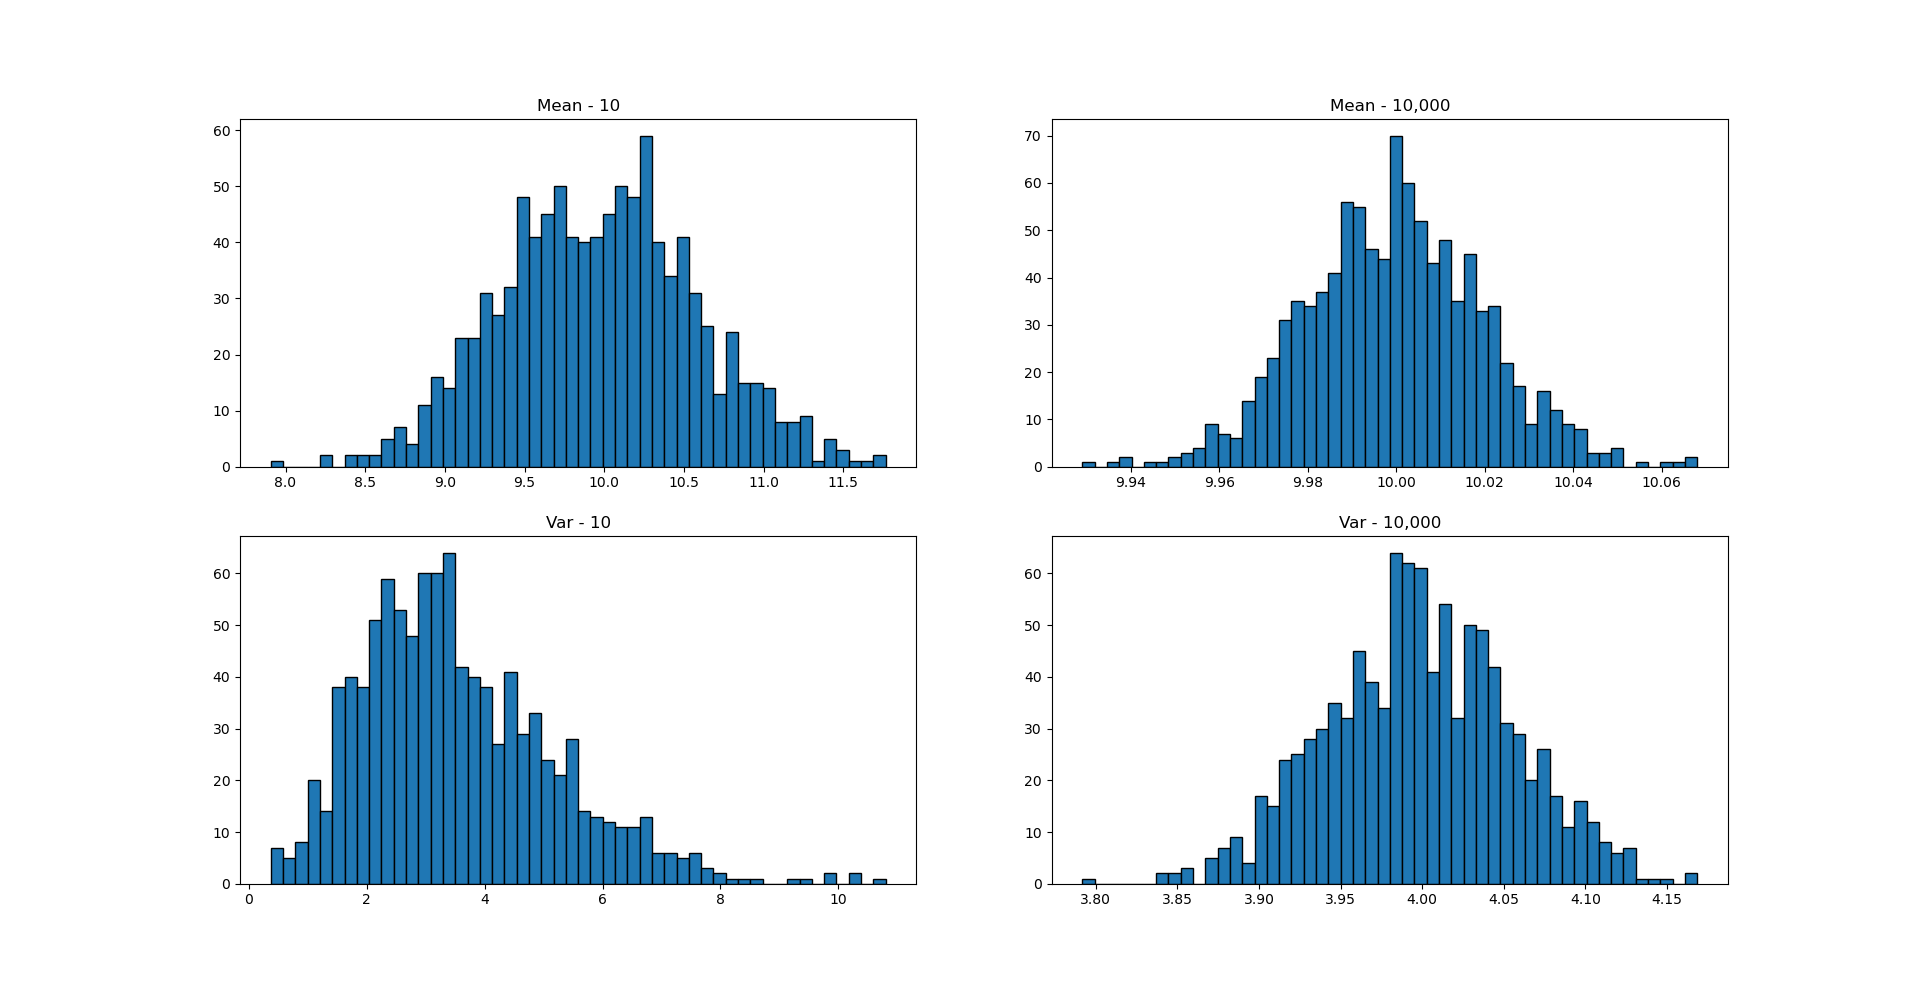
\includegraphics[width = 0.5\textwidth]{inc/p1_hist.png}

The figures above show the results of estimating the mean and variance from Gaussian RV, at 10 and 10,000 realisations. With greater N of realisations the mean is seen to converge symmetrically around the parameter where the variance is cantered left and tails off, ie right skewed.

\subsubsection*{Part 2}
\begin{center}
        Imported sound data from Speech.pcm
        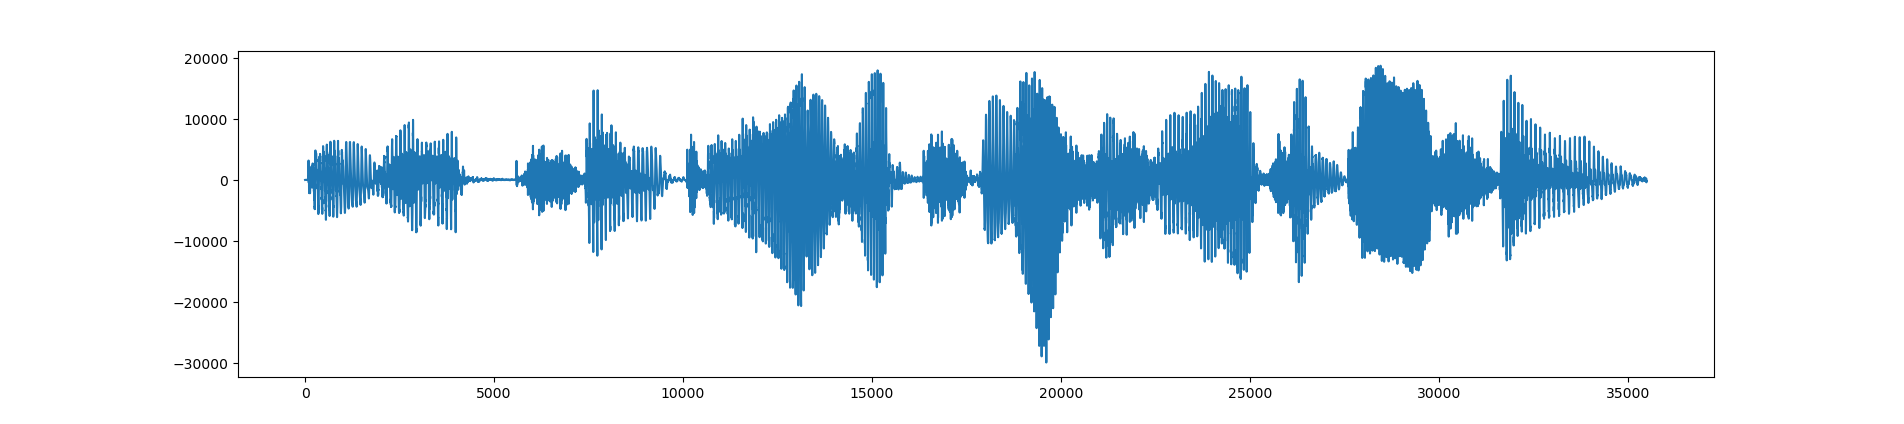
\includegraphics[width = \textwidth]{inc/data.png} 
\end{center}

Implementing the theory (outlined above) with python to maximise the likelihood equation and repeating until convergence produce the final values:
$$\alpha = 0.7119 \hspace*{64pt} \beta = 1755.1$$

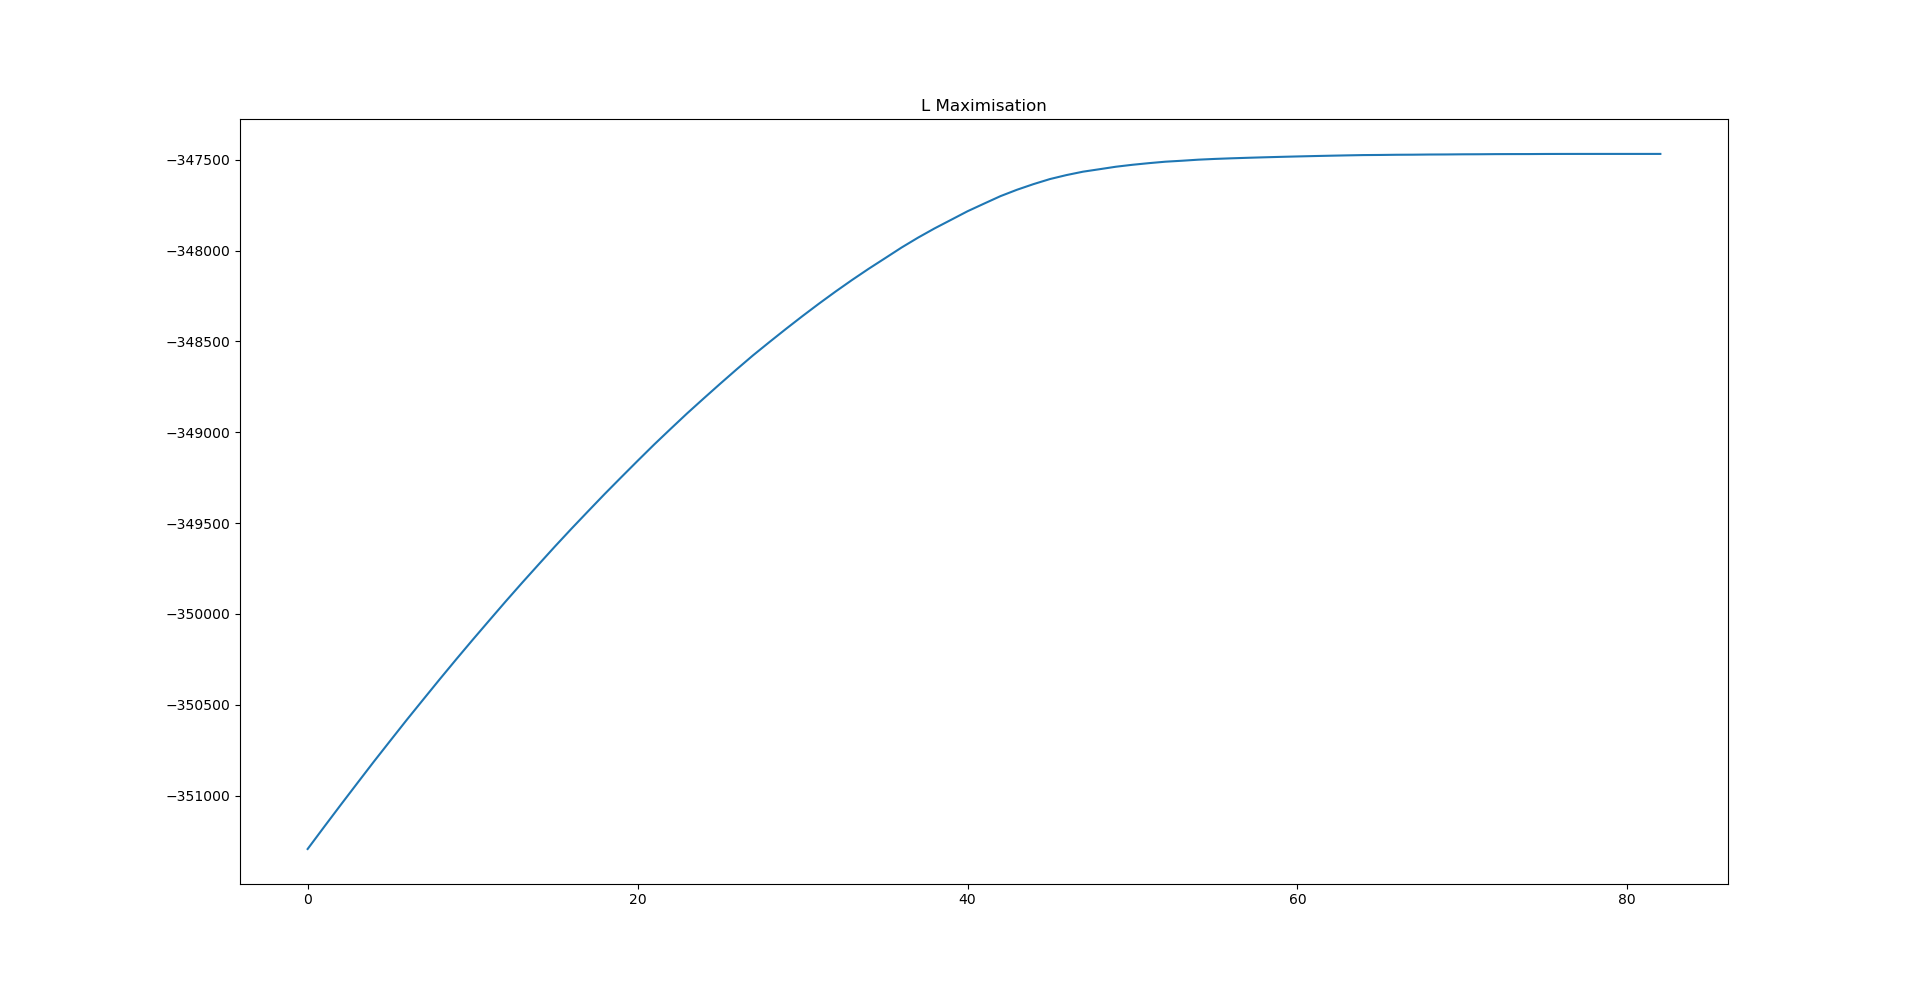
\includegraphics[width = 0.5\textwidth]{inc/L-maxed.png}
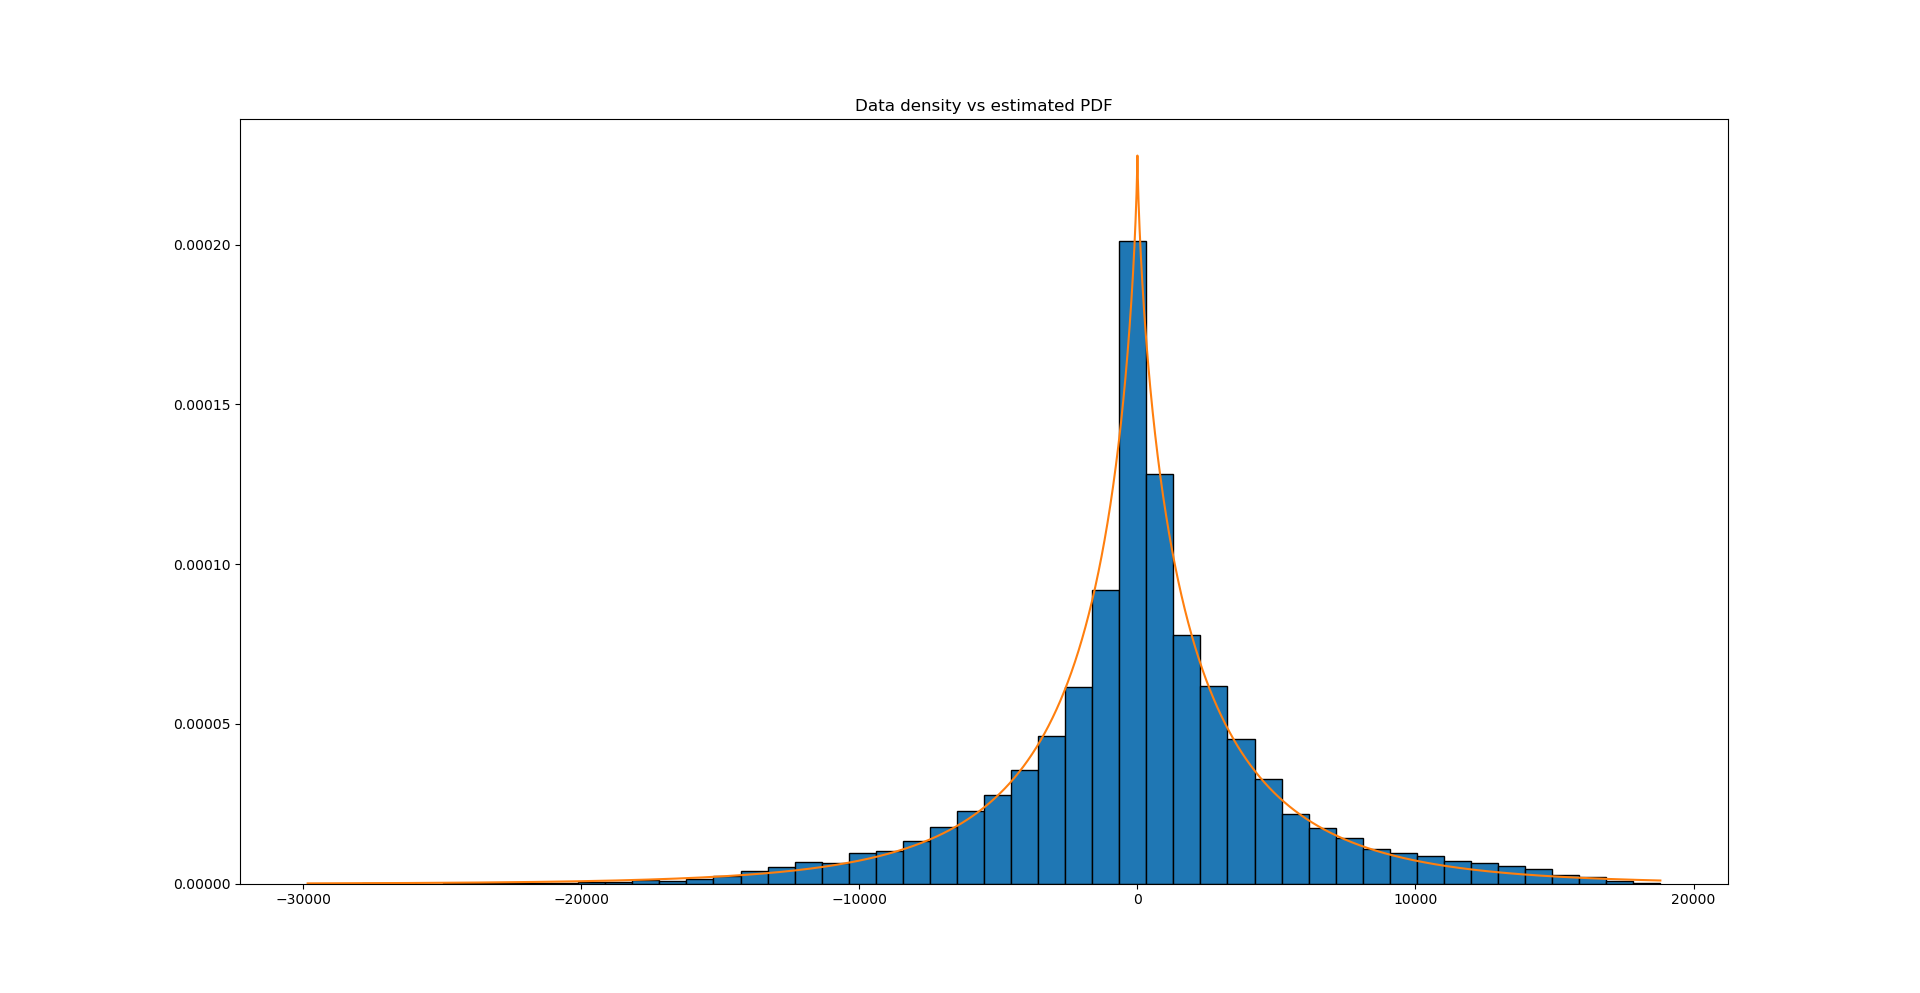
\includegraphics[width = 0.5\textwidth]{inc/densityVpdf.png} 

The figure right show the maximisation of the ln(likelihood) equation as the algorithm progressed and the figure right show the density histogram of the signal overlaid with the computed theoretical pdf using the estimated parameters; showing the success of this estimation method.

Note: The outer loop only iterated 83 times before convergence.

\Newpage
\section*{Appendix}
\subsection*{Part 1}
\inputpython{../py/lab3_1.py}{1}{100}
\subsection*{Part 2}
\inputpython{../py/lab3_2.py}{1}{100}

\end{preview}
\end{document}